\vspace{-0.3em}
\subsection {Case study: DCQCN versus TIMELY on flow completion time}
\label{sec:fct}

While we show that both ECN-based DCQCN and delay-based TIMELY can be 
stable and fair if properly tuned (see Section~\ref{sec:dcqcn} and 
Section~\ref{sec:timely}), they may differ on other important performance
metrics. For example, the end users often care about flow completion
times, especially for short flows~\cite{rcp}. We compare the flow completion 
times of DCQCN and TIMELY with 
a simple simulation, using the classic dumbbell topology shown in
Figure~\ref{fig:fct_topo}. The topology consists of 20 nodes -- 10 senders and
10 receivers. All traffic flows across the bottleneck link between the two
switches, SW1 and SW2. All links are 10Gbps with 1$\mu$s latency.

The traffic consists  of long and short-lived flows, between pairs of randomly
selected sender and receiver nodes. The flow size distribution is derived from
the traffic distribution reported in~\cite{dctcp}. The interarrival time of
flows is picked from am exponential distribution. The load on the bottleneck
link is varied by changing the mean of the distribution. This traffic generation
model was also used in several recent studies, including pFabric~\cite{pfabric}
and ProjecToR~\cite{projector}. 

Both DCQCN and TIMELY used the default parameter settings recommended
in~\cite{dcqcn} and ~\cite{timely}, respectively. 
The metric of interest is the flow completion time of small flows. Following 
pFabric~\cite{pfabric}, we define small flows as flows that send fewer than 100KB. 
We also tune and test different protocol parameter and small flow threshold settings. 
The results are similar.

Figure~\ref{fig:fct_results} shows the median and 90th percentile of FCT and
DCQCN, TIMELY original and patched TIMELY as the load is varied. Patched TIMELY is our 
modification to TIMELY's protocol to ensure a unique fixed point (\S\ref{sec:timely_fixed}). 
The X axis shows relative load: load factor of 1 corresponds to an average of 8Gbps of traffic 
on the bottleneck link. The scaling is linear. We see that at higher loads, FCT for both TIMELY 
and patched TIMELY is high, and highly variable. This illustrated in detail in 
Figure~\ref{fig:fct_cdf}, which shows the CDF of the flow completion time for
load factor of 0.8. 

The reason for TIMELY's poor performance is evident from
Figure~\ref{fig:fct_queue}, which shows the queue length at the link between
SW1 and SW2 for a load factor of 0.8. As shown, the queue length under TIMELY
can grow to a very high value, and is highly variable. In contrast the DCQCN queue has a
fixed point between the RED thresholds and even in the transient state
the queue stays within the bounds. Note that patched TIMELY is operating in between the original 
TIMELY protocol and DCQCN. This is because our fix is ensuring a
unique fixed point (and thus fairness), without 
changing the dynamics of TIMELY's queue build up. 
%\fixme{We argue that this is due
%to fundamental limits of using delay as the congestion signal, as discussed in 
%Section~\ref{sec:ecn_advantages}.}

\begin{figure*}[t]
\centering
\mbox{
\begin{minipage}{0.32\textwidth}
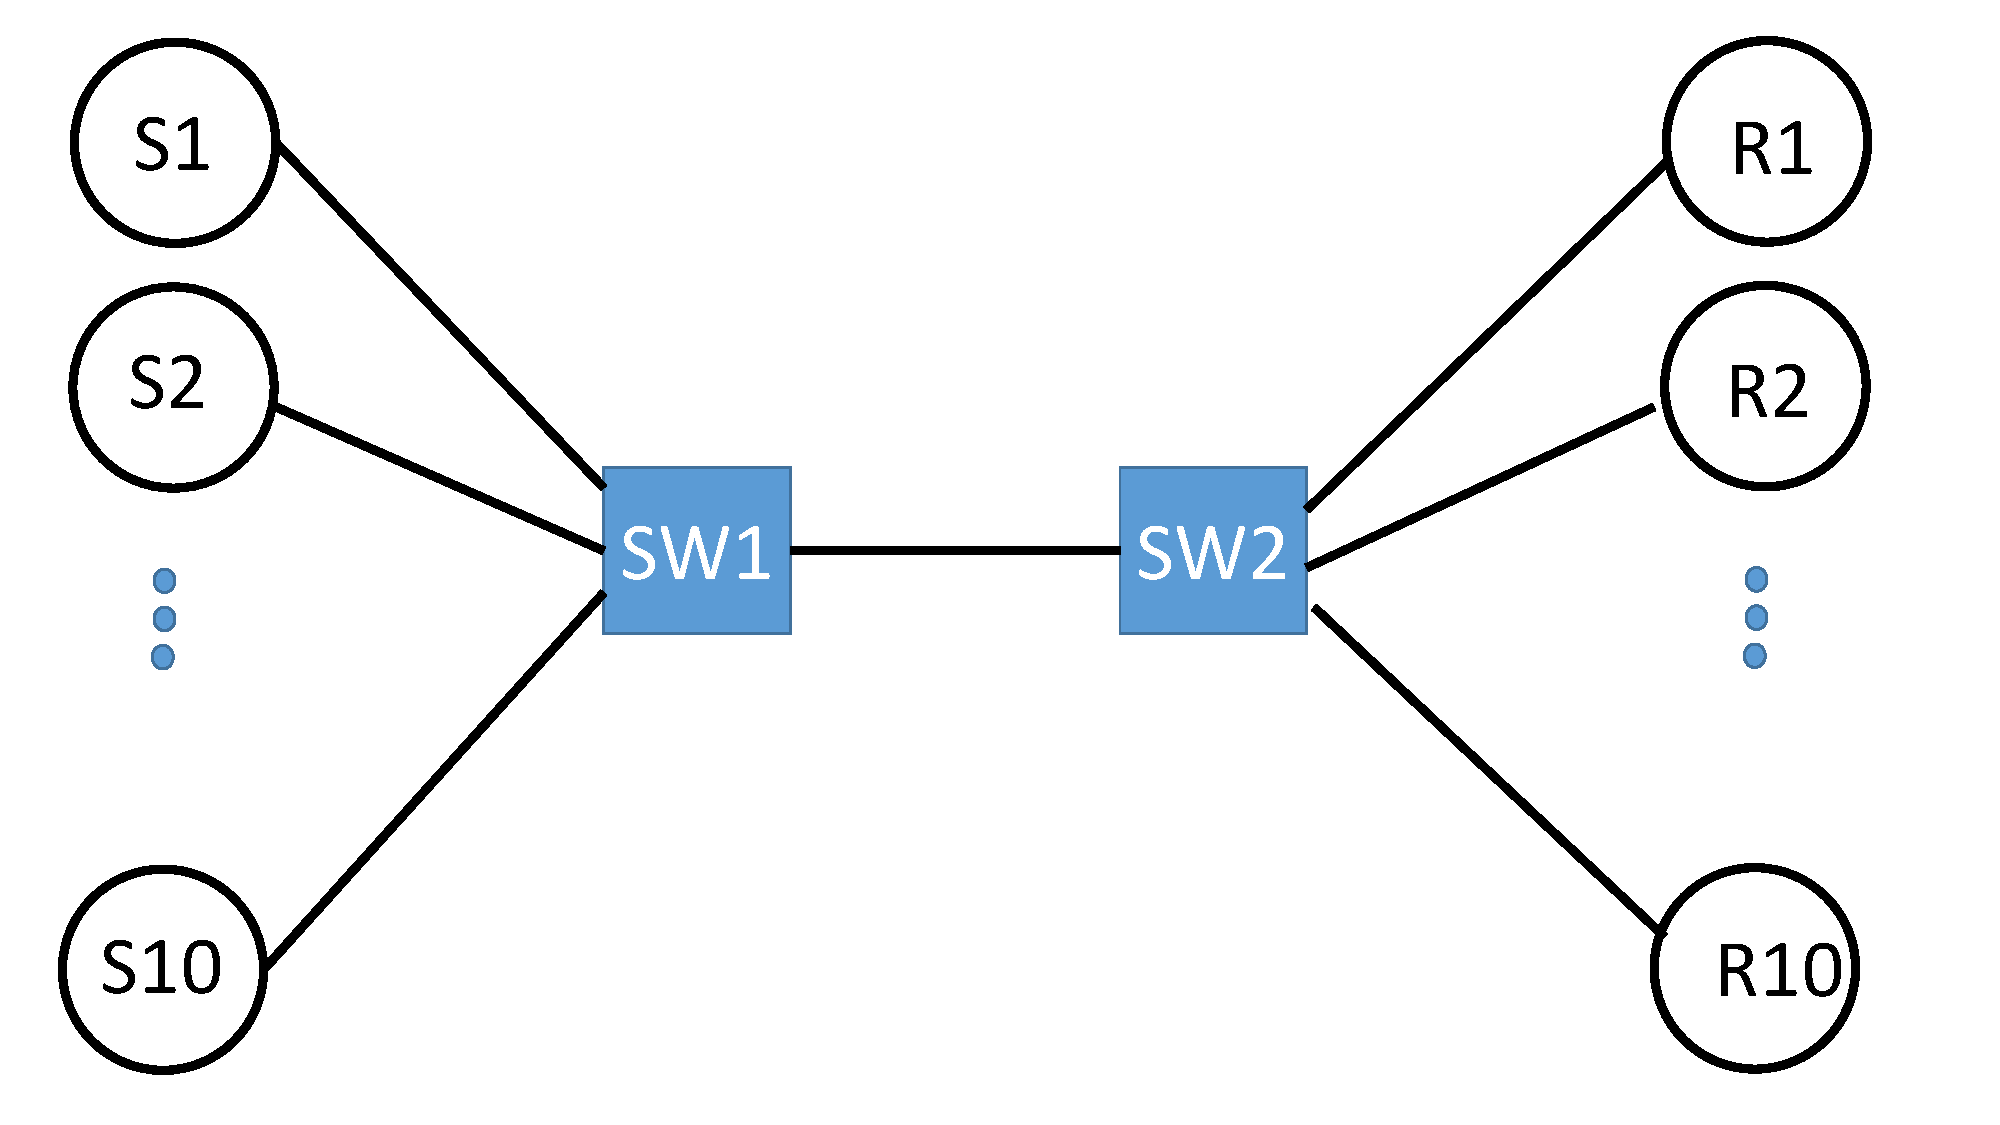
\includegraphics[width=0.99\textwidth]{figures/dumbbell.pdf}
\vspace{-1em}
\caption{The dumbbell topology. All links are 10Gbps with 1$\mu$s latency.}
\vspace{-1em}
\label{fig:fct_topo}
\end{minipage}
\quad
\begin{minipage}{0.62\textwidth}
\subfigure{ 
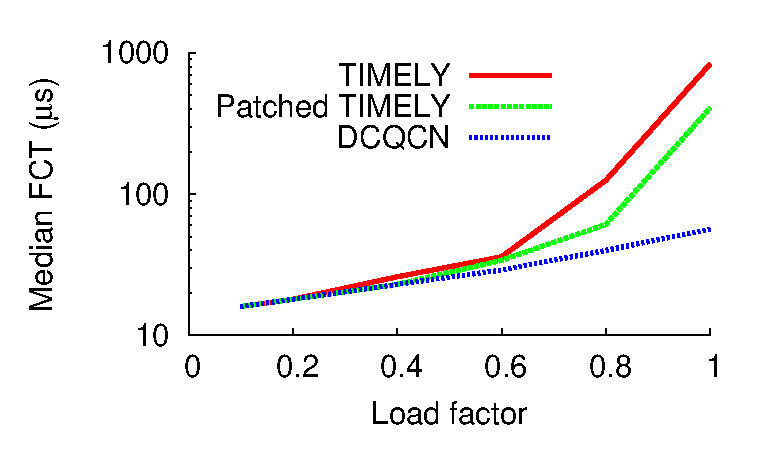
\includegraphics[width=0.48\textwidth]{figures/fct_median.eps}
\label{fig:fct_median}
}
\subfigure{ 
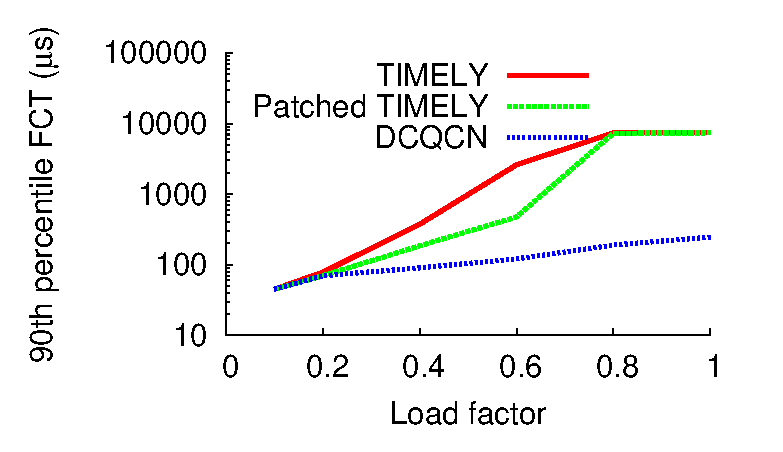
\includegraphics[width=0.48\textwidth]{figures/fct_90.eps}
\label{fig:fct_90}
}
\vspace{-1em}
\caption{Median and 90th percentile of FCT of small flows. Note log scale on Y axis.}
\vspace{-1em}
\label{fig:fct_results}
\end{minipage}
}
\end{figure*}

\if 0
\begin{figure}[t]
\center
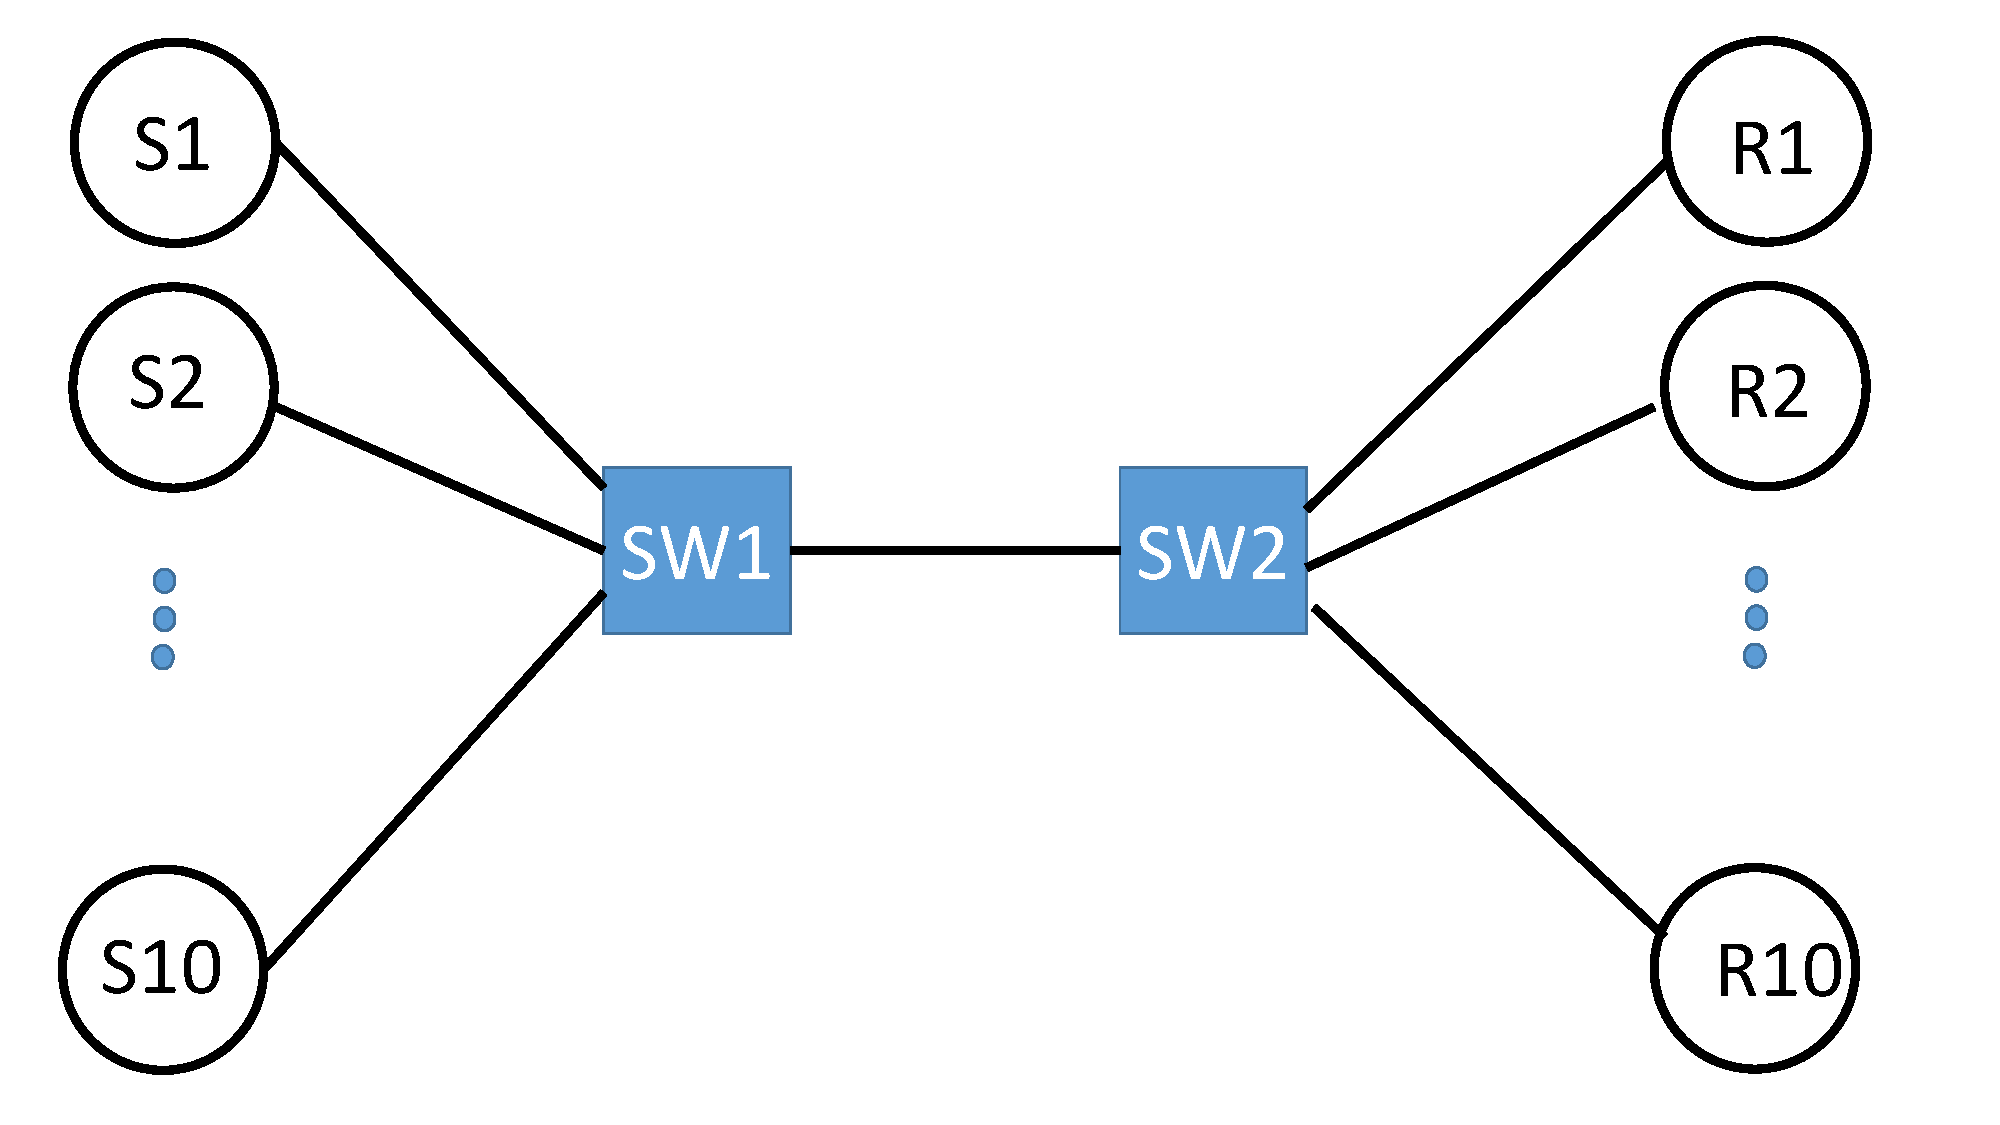
\includegraphics[width=0.3\textwidth]{figures/dumbbell.pdf}
\caption{The dumbbell toplogy. All links are 10Gbps with 1$\mu$s latency.}
\label{fig:fct_topo}
\end{figure}

\begin{figure}[t]
\center
\subfigure []{ 
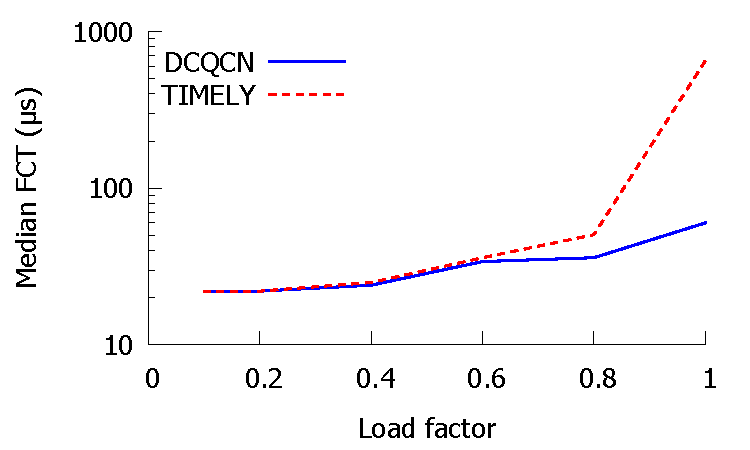
\includegraphics[width=0.3\textwidth]{figures/fct_median.pdf}
\label{fig:fct_median}
}
\subfigure []{ 
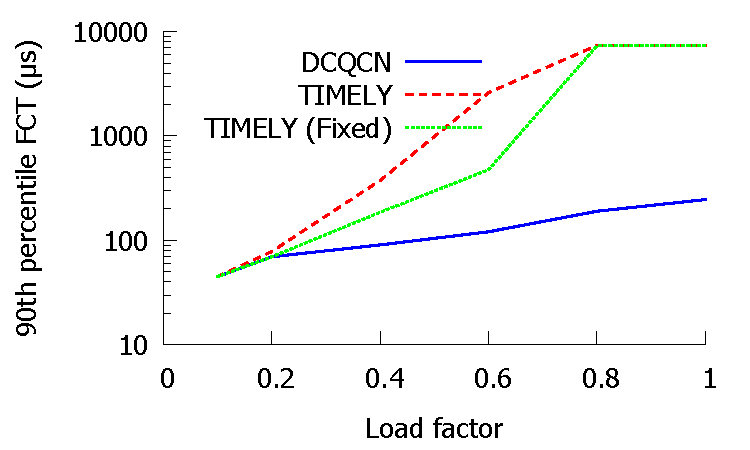
\includegraphics[width=0.3\textwidth]{figures/fct_90.pdf}
\label{fig:fct_90}
}
\caption{Median and 90th percentile of FCT of small flows. Note log scale on Y axis.}
\label{fig:fct_results}
\end{figure}
\fi


\begin{figure*}[t]
\centering
\mbox{
\begin{minipage}{0.32\textwidth}
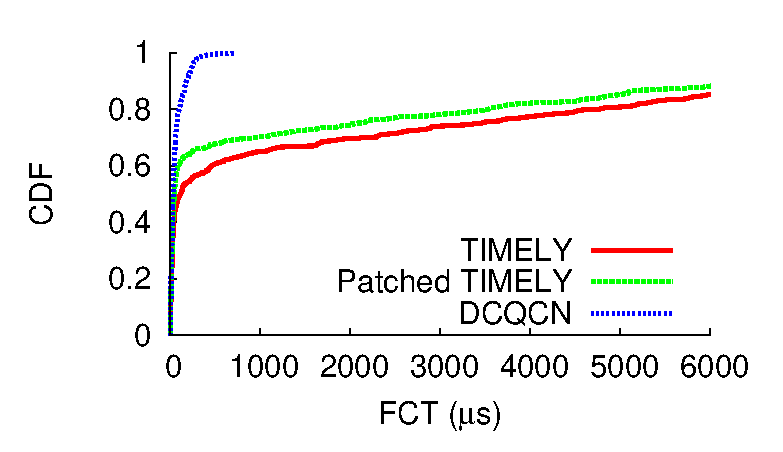
\includegraphics[width=0.99\textwidth]{figures/fct_cdf.eps}
\caption{CDF of FCT for load=0.8}
\vspace{-1.5em}
\label{fig:fct_cdf}
\end{minipage}
\quad
\begin{minipage}{0.34\textwidth}
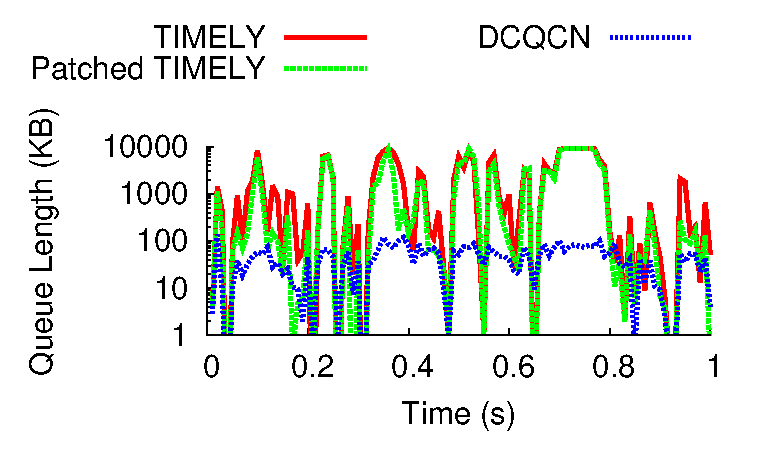
\includegraphics[width=0.99\textwidth]{figures/fct_queue.eps}
\caption{Bottleneck Queue for load=0.8. Note log scale on Y axis.}
\vspace{-1em}
\label{fig:fct_queue}
\end{minipage}
\quad
\begin{minipage}{0.29\textwidth}
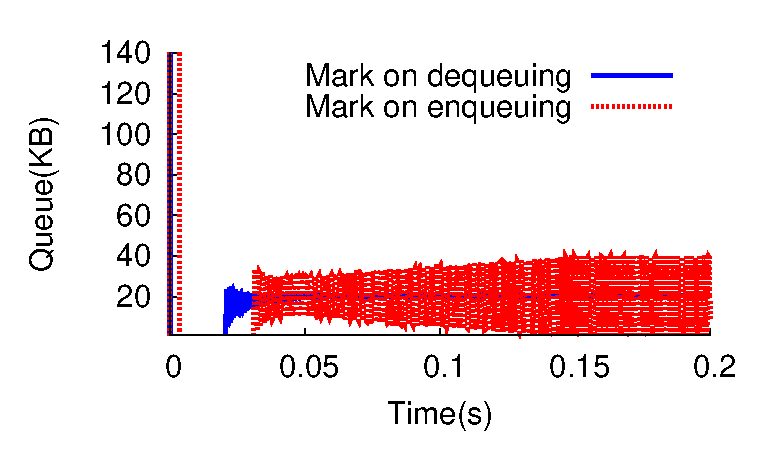
\includegraphics[width=0.99\textwidth]{figures/dcqcn_bufferbloat.eps}
\vspace{-2em}
\caption{DCQCN stability when two flows compete for a 
bottleneck with 85$\mu$s feedback delay.}
\vspace{-2em}
\label{fig:dcqcn_bufferbloat}
\end{minipage}
}
\end{figure*}

\if 0
\begin{figure}[t]
\center
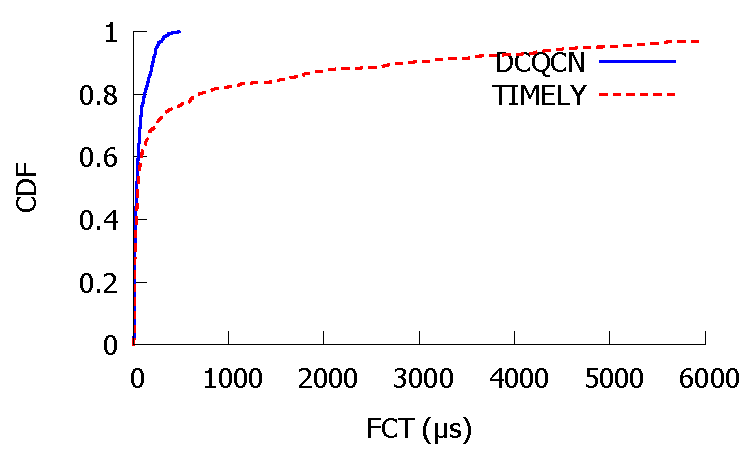
\includegraphics[width=0.3\textwidth]{figures/fct_cdf.pdf}
\caption{CDF of FCT for load=0.8}
\label{fig:fct_cdf}
\end{figure}

\begin{figure}[t]
\center
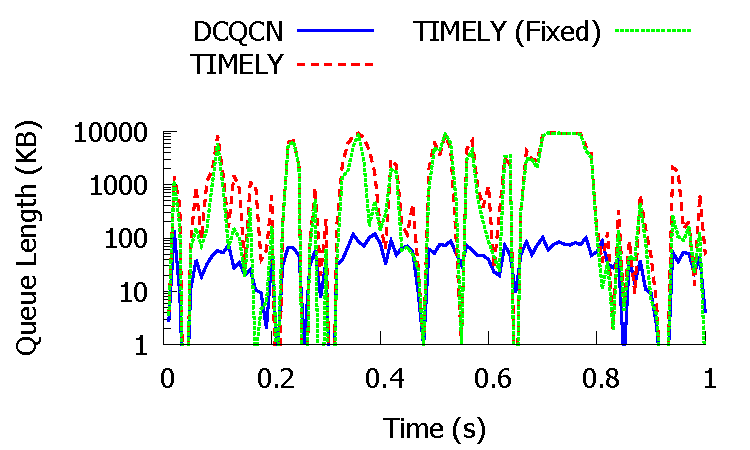
\includegraphics[width=0.3\textwidth]{figures/fct_queue.pdf}
\caption{Bottleneck Queue for load=0.8. Note log scale on Y axis.}
\label{fig:fct_queue}
\end{figure}
\fi

We note that in all cases, the link utilization is roughly the same for DCQCN
and TIMELY, indicating that the long flows performed similarly with both
schemes.
